\begin{frame}
    \begin{centering}
        \vskip5ex plus 1filll
        {\usebeamerfont{title page title}\usebeamercolor[fg]{title page} Nonlinear Filters\\[1.5ex]}
        \vskip0pt plus 1filll
    \end{centering}
\end{frame}

\begin{frame}{Biquad Filter}
    Transposed Direct Form II
    \begin{figure}
        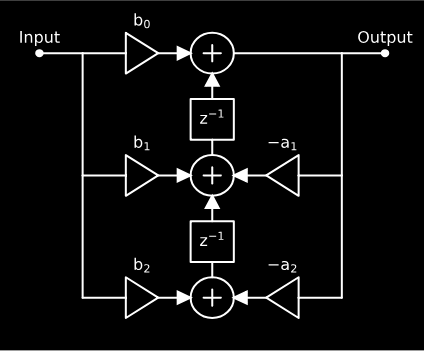
\includegraphics[height=2.5in]{../NonlinearBiquad/Pics/TDF-II.png}
    \end{figure}
\end{frame}

\begin{frame}{Biquad Filter}
    Difference equation:
    \begin{equation}
        y[n] = b_0 u[n] + b_1 u[n-1]
        + b_2 u[n-2] - a_1 y[n-1]
        - a_2 y[n-2]
    \end{equation}

    State space formulation:
    \begin{equation}
        \begin{bmatrix} x_1[n+1] \\ x_2[n+1] \\ y[n+1] \end{bmatrix} =
        \begin{bmatrix} 0& 1& -a_1\\ 0& 0& -a_2\\ 1& 0& 0 \end{bmatrix}
        \begin{bmatrix} x_1[n] \\ x_2[n] \\ y[n] \end{bmatrix}
        + \begin{bmatrix} b_1\\ b_2\\ b_0 \end{bmatrix} u[n]
    \end{equation}
\end{frame}

\begin{frame}{Nonlinear Biquad Filter}
    \begin{figure}
        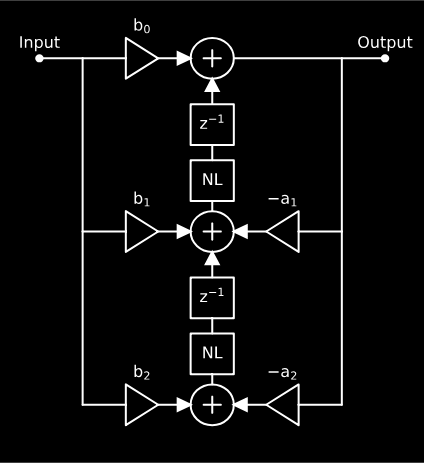
\includegraphics[height=2.5in]{../NonlinearBiquad/Pics/NL-TDF-II.png}
    \end{figure}
\end{frame}

\begin{frame}{Nonlinear Biquad Filter}
    Saturating nonlinearities \rightarrow nonlinear resonance
    \begin{figure}
        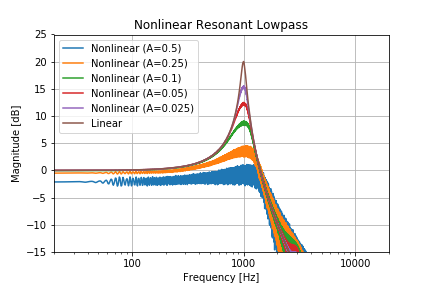
\includegraphics[height=2.5in]{../NonlinearBiquad/Pics/NL-LPF.png}
    \end{figure}
\end{frame}

\begin{frame}{Nonlinear Biquad Filter}
    Saturating nonlinearities \rightarrow nonlinear resonance
    \begin{figure}
        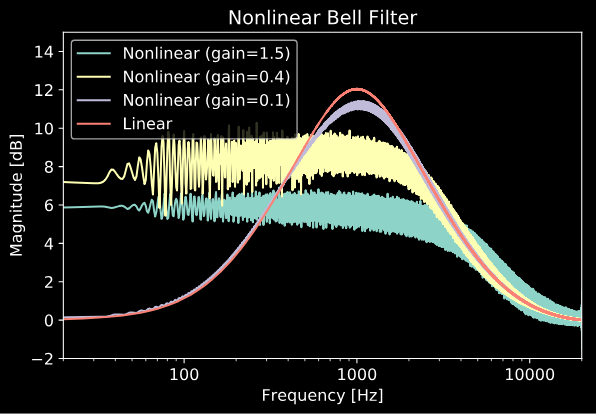
\includegraphics[height=2.5in]{../NonlinearBiquad/Pics/NL-Bell.png}
    \end{figure}
\end{frame}

\begin{frame}{Nonlinear Biquad Filter}
    Saturating nonlinearities \rightarrow nonlinear resonance
    \begin{figure}
        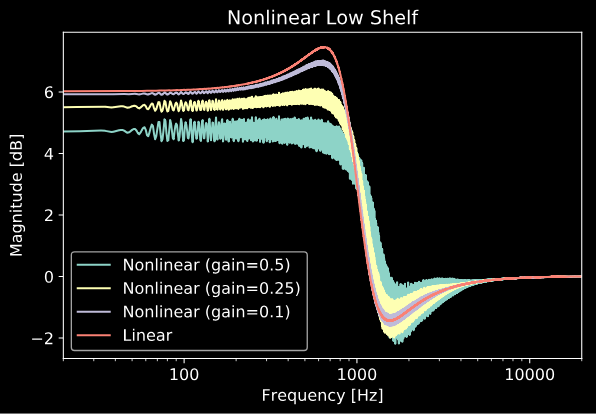
\includegraphics[height=2.5in]{../NonlinearBiquad/Pics/NL-LowShelf.png}
    \end{figure}
\end{frame}

\begin{frame}{Nonlinear Biquad Filter}
    Pole/zero movement
    \begin{figure}
        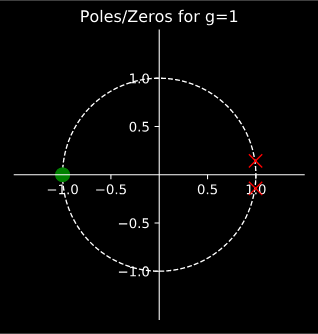
\includegraphics[width=1.33in]{../NonlinearBiquad/Pics/pz1.png}
        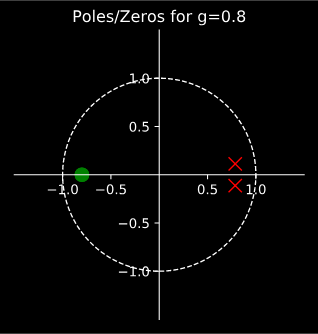
\includegraphics[width=1.33in]{../NonlinearBiquad/Pics/pz08.png}
        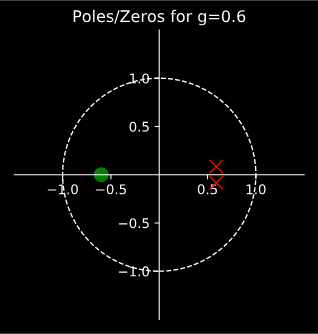
\includegraphics[width=1.33in]{../NonlinearBiquad/Pics/pz06.png}
        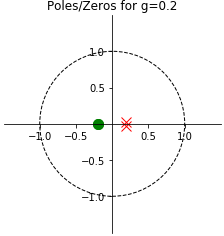
\includegraphics[width=1.33in]{../NonlinearBiquad/Pics/pz02.png}
    \end{figure}
\end{frame}

\begin{frame}{Nonlinear Feedback Filter}
    \begin{figure}
        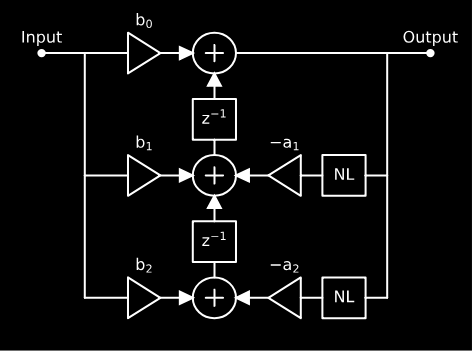
\includegraphics[height=2.5in]{../NonlinearFeedback/Pics/NL2-TDF-II.png}
    \end{figure}
\end{frame}

\begin{frame}{Nonlinear Feedback Filter}
    Saturating nonlinearity \rightarrow cutoff frequency modulation
    \begin{figure}
        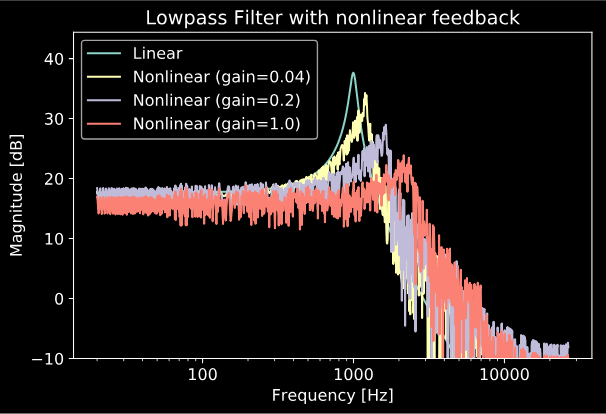
\includegraphics[height=2.5in]{../NonlinearFeedback/Pics/LPF-NL.png}
    \end{figure}
\end{frame}

\begin{frame}{Nonlinear Feedback Filter}
    Pole/zero movement
    \begin{figure}
        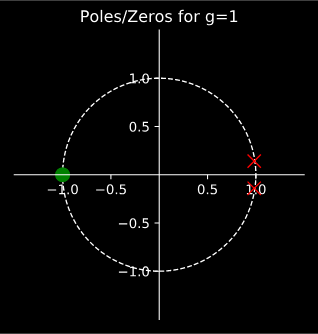
\includegraphics[width=1.33in]{../NonlinearFeedback/Pics/pz1.png}
        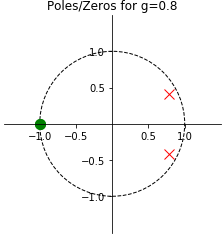
\includegraphics[width=1.33in]{../NonlinearFeedback/Pics/pz08.png}
        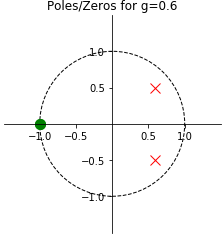
\includegraphics[width=1.33in]{../NonlinearFeedback/Pics/pz06.png}
        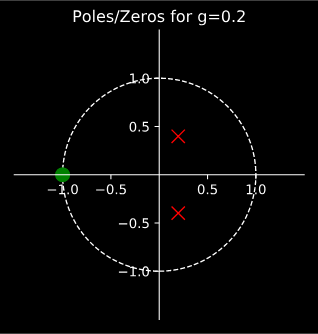
\includegraphics[width=1.33in]{../NonlinearFeedback/Pics/pz02.png}
    \end{figure}
\end{frame}

\begin{frame}{Nonlinear Biquad Stability}
    \textbf{Questions:}\newline\newline
    Can we guarantee that a nonlinear filter will be stable
    given that its linear corrolary is stable?
    \newline\newline
    For what subset of nonlinear functions is this guaranteed?
\end{frame}

\begin{frame}{Nonlinear Biquad Stability}
    Test case: saturating nonlinearity, $f_{NL} = \tanh(x)$ \rightarrow STABLE!
    \begin{figure}
        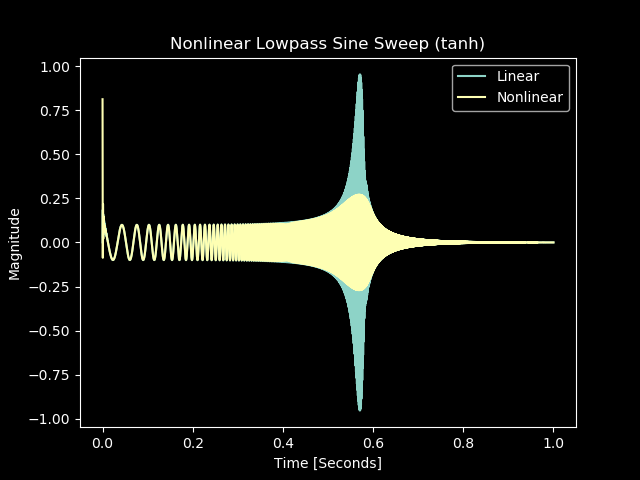
\includegraphics[height=2.5in]{Figures/nl_lpf_stable.png}
    \end{figure}
\end{frame}

\begin{frame}{Nonlinear Biquad Stability}
    Test case: full wave rectifier, $f_{NL} = 0.45 |x|$ \rightarrow UNSTABLE!
    \begin{figure}
        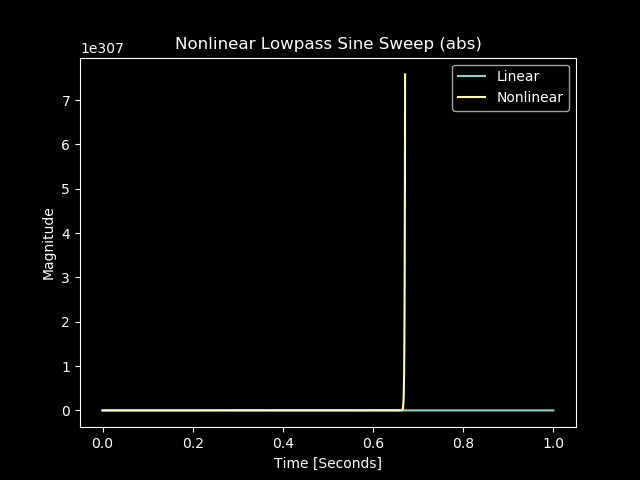
\includegraphics[height=2.5in]{Figures/nl_lpf_unstable.png}
    \end{figure}
\end{frame}

\begin{frame}{Nonlinear Biquad Stability}
    Test case: sine, $f_{NL} = \sin (x)$ \rightarrow STABLE!
    \begin{figure}
        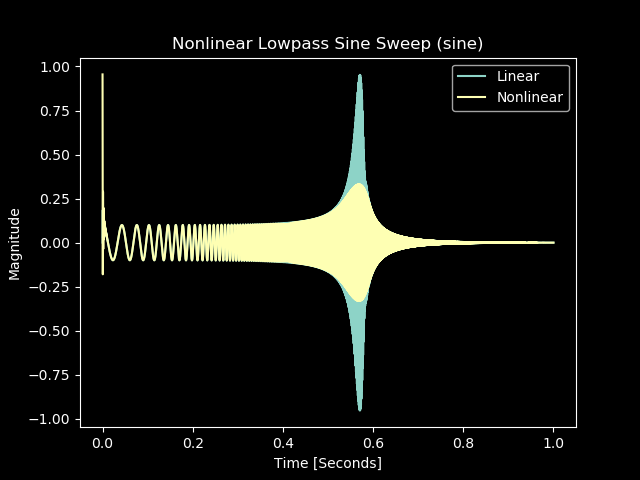
\includegraphics[height=2.5in]{Figures/nl_lpf_sine.png}
    \end{figure}
\end{frame}

\begin{frame}{Lyapunov Stability\footcite{Lyapunov}}
    1. Form state space equation:
    \begin{equation}
        \mathbf{x}[n+1] = \mathbf{f}(\mathbf{x}[n])
    \end{equation}
    2. Find Jacobian $\mathbf{J}$ of $\mathbf{f}$
    \newline\newline
    3. If every element of $\mathbf{J}$ is less than 1
    at some operating point, the system is Lyapunov
    stable about that point.
\end{frame}

\begin{frame}{Nonlinear Biquad Stability}
    \begin{equation}
        \begin{bmatrix} x_1[n+1] \\ x_2[n+1] \\ y[n+1] \end{bmatrix} =
        \mathbf{h} \left( \begin{bmatrix} x_1[n] \\ x_2[n] \\ y[n] \end{bmatrix}
        \right) + \begin{bmatrix} b_1\\ b_2\\ b_0 \end{bmatrix} u[n]
    \end{equation}
    \vspace{3ex}
    \begin{equation}
        \begin{split}
            h_1(x_1[n], x_2[n], y[n]) =& f_{NL}(x_2[n]) - a_1y[n] \\
            h_2(x_1[n], x_2[n], y[n]) =& -a_2y[n] \\
            h_3(x_1[n], x_2[n], y[n]) =& f_{NL}(x_1[n])
        \end{split}
    \end{equation}
\end{frame}

\begin{frame}{Nonlinear Biquad Stability}
    \begin{equation}
        \mathbf{J} = \begin{bmatrix}
            0& f'_{NL}(x_2[n])& -a_1 \\
            0& 0& -a_2 \\
            f'_{NL}(x_1[n])& 0& 0
        \end{bmatrix}
    \end{equation}

    \vspace{3ex}

    Note that if $f'_{NL}$ does not exist at some point,
    the system is NOT stable at that point.
\end{frame}

\begin{frame}{Nonlinear Feedback Stability}
    \begin{equation}
        \begin{bmatrix} x_1[n+1] \\ x_2[n+1] \\ y[n+1] \end{bmatrix} =
        \mathbf{h} \left( \begin{bmatrix} x_1[n] \\ x_2[n] \\ y[n] \end{bmatrix}
        \right) + \begin{bmatrix} b_1\\ b_2\\ b_0 \end{bmatrix} u[n]
    \end{equation}
    \vspace{3ex}
    \begin{equation}
        \begin{split}
            h_1(x_1[n], x_2[n], y[n]) =& x_2[n] - a_1f_{NL}(y[n]) \\
            h_2(x_1[n], x_2[n], y[n]) =& -a_2f_{NL}(y[n]) \\
            h_3(x_1[n], x_2[n], y[n]) =& x_1[n]
        \end{split}
    \end{equation}
\end{frame}

\begin{frame}{Nonlinear Feedback Stability}
    \begin{equation}
        \mathbf{J} = \begin{bmatrix}
            0& 1& -a_1f'_{NL}(y[n]) \\
            0& 0& -a_2f'_{NL}(y[n]) \\
            1& 0& 0
        \end{bmatrix}
    \end{equation}
\end{frame}

\begin{frame}{Nonlinear Biquad Stability}
    General stability contstraint:
    \begin{equation}
        |f'_{NL}(x)| \leq 1
    \end{equation}
    \newline\newline
    \small
    Note: if the $f'_{NL}(x)$ does not exist, the filter is not guaranteed stable.
\end{frame}

\begin{frame}{Nonlinear Biquad Stability}
    If derivative doesn't exist at every point: use BLAMP\footcite{BLAMP}!
    \begin{figure}
        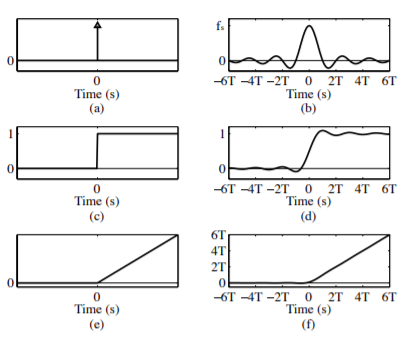
\includegraphics[height=2.2in]{Figures/blamp.png}
    \end{figure}
\end{frame}

\begin{frame}{Nonlinear Biquad Filter}
    Can we use this for analog modelling?
    \begin{figure}
        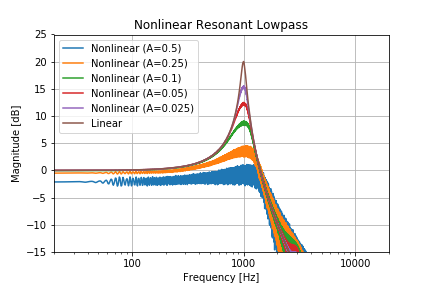
\includegraphics[height=2.5in]{../NonlinearBiquad/Pics/NL-LPF.png}
    \end{figure}
\end{frame}

\begin{frame}{Nonlinear Biquad Filter}
    Parameters: nonlinearities, input gain
    \begin{figure}
        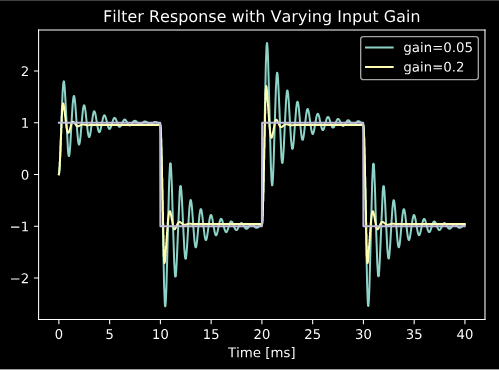
\includegraphics[height=2.5in]{../NonlinearBiquad/Pics/50-Hz_Response.png}
    \end{figure}
\end{frame}

\begin{frame}{Nonlinear Biquad Filter}
    Modelling an overdriven Sallen-Key lowpass filter
    \begin{figure}
        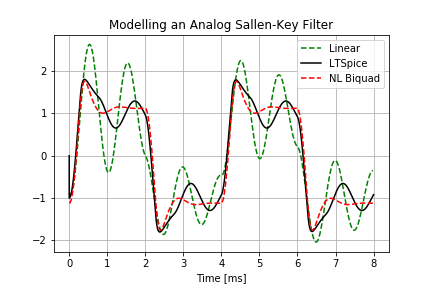
\includegraphics[height=2.5in]{../NonlinearBiquad/Pics/Spice-Compare.png}
    \end{figure}
\end{frame}
